%&pdflatex
\section{Bootloader e primo avvio}
L'ultimo passo è l'installazione del \textit{bootloader} (\texttt{GRUB}).

Senza un bootloader, Debian non potrebbe avviarsi. Quindi consigliamo di installare \texttt{GRUB} (bisogna rispondere \texttt{Yes} (\texttt{Sì}) alla domanda mostrata in Figura \vref{fig:install-grub}).

\begin{figure}[ht]
	\centering
	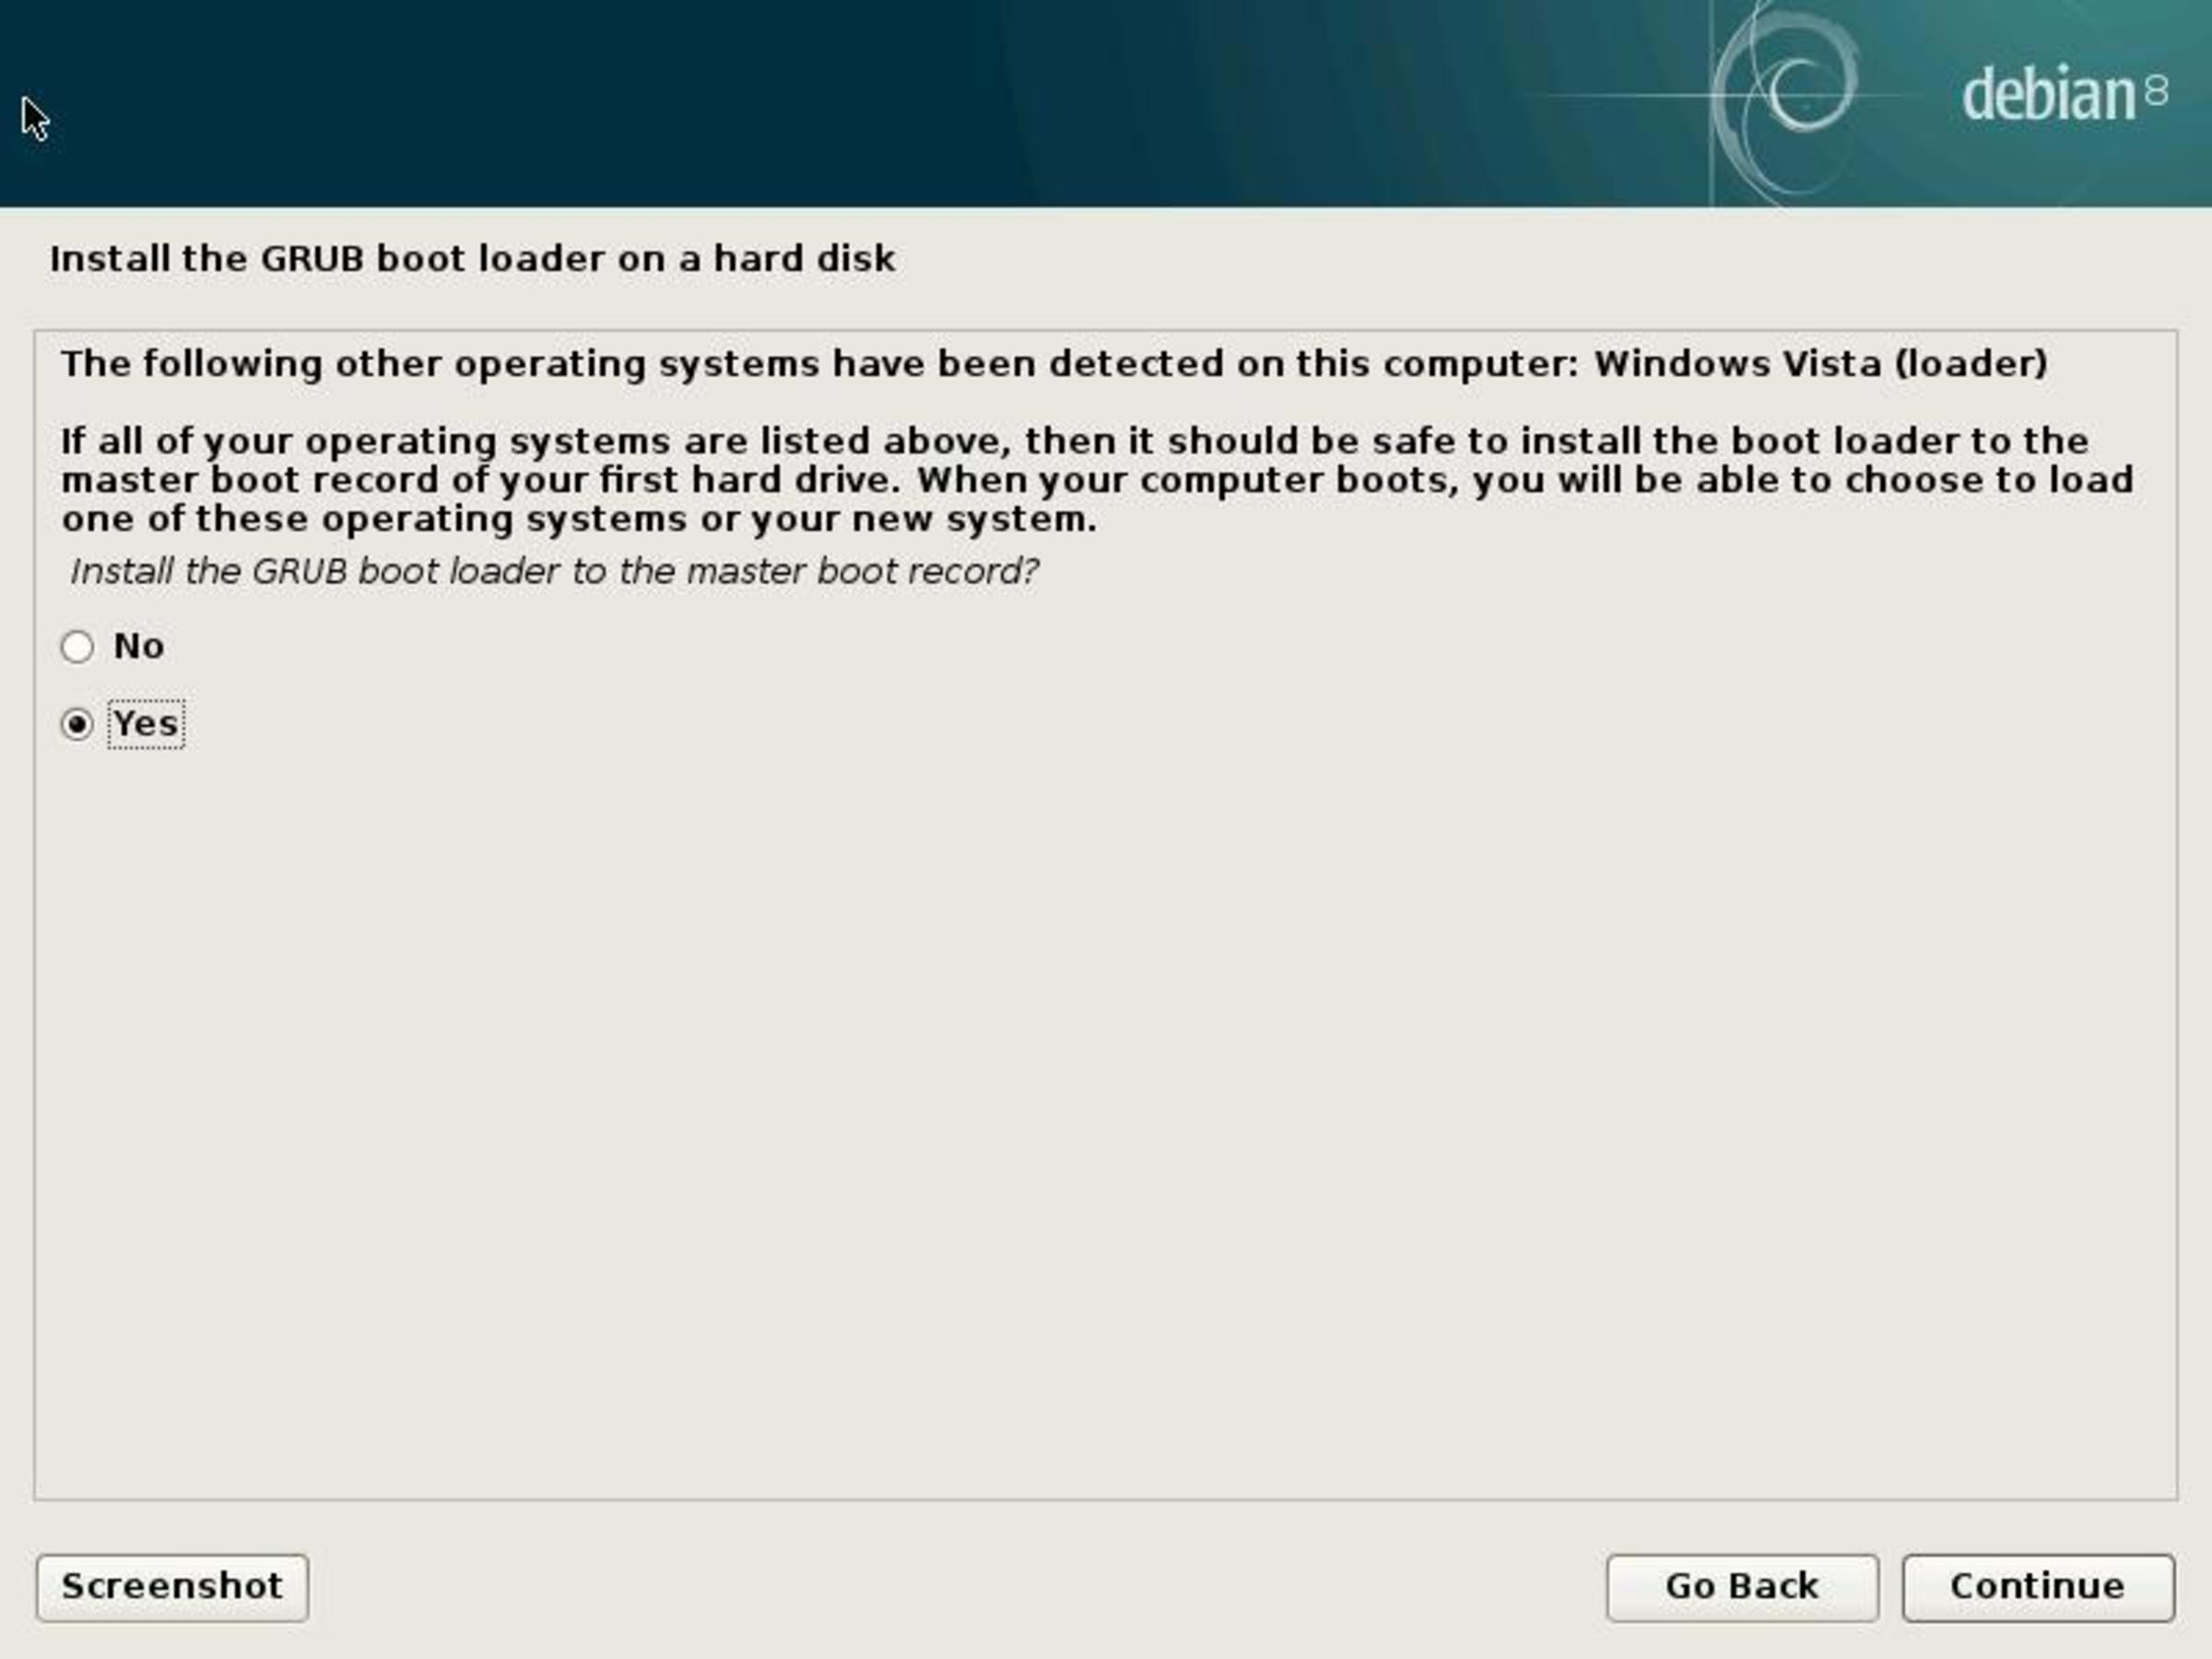
\includegraphics[resolution=600]{install-grub}
	\caption{Installazione di \texttt{GRUB}}
	\label{fig:install-grub}
\end{figure}

Nella schermata successiva, dobbiamo scegliere il disco sul quale si desidera installare \texttt{GRUB}. Si scelga il disco più adatto (di solito, lo stesso su cui si è installato Debian).

Infine, Debian ci chiede di rimuovere il disco di installazione del sistema. Rimuoviamo il disco (o il pendrive USB) e riavviamo cliccando su \texttt{Continue} (\texttt{Continua}).

Al riavvio, se tutto è andato per il meglio, dovrebbe comparire la schermata di \texttt{GRUB} mostrata in Figura \vref{fig:grub}.

\begin{figure}[ht]
	\centering
	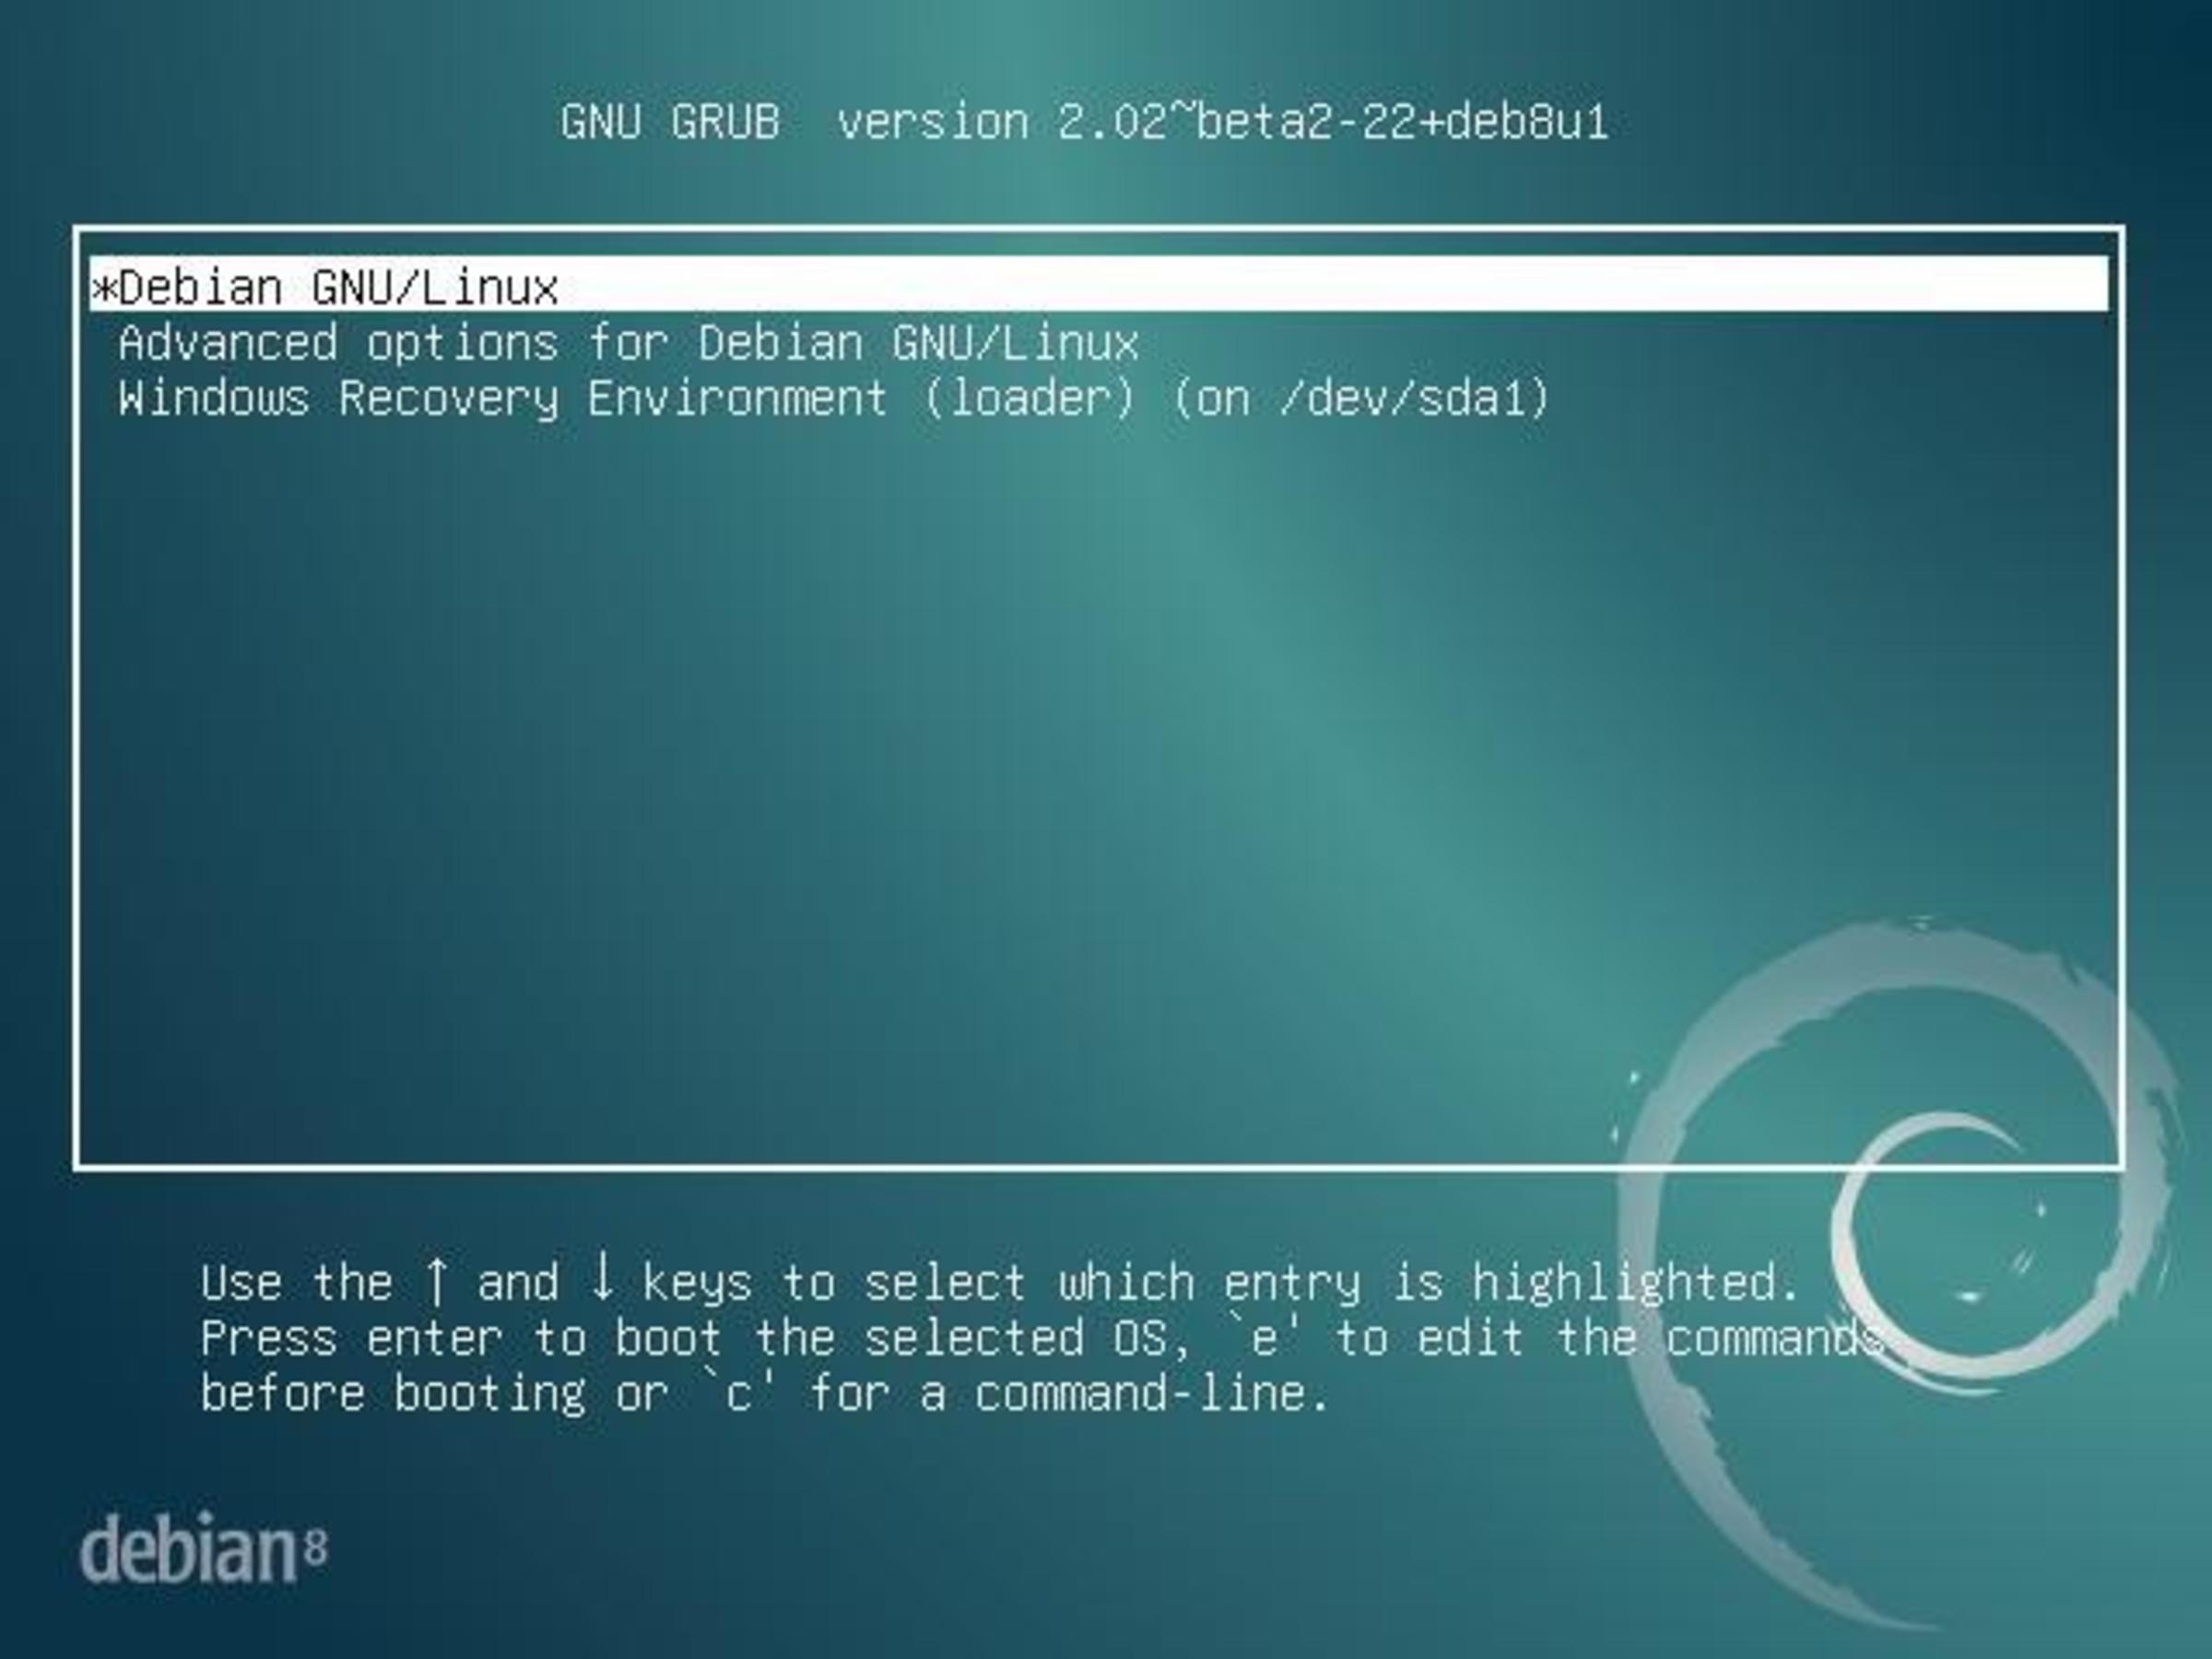
\includegraphics[resolution=600]{grub}
	\caption{Selezione del sistema operativo da avviare con \texttt{GRUB}}
	\label{fig:grub}
\end{figure}


Per avviare Debian, sceglieremo la prima voce. La terza voce altro non è che Windows 10 con un nome un po' fuorviante.

Se tutto funziona, Debian dovrebbe avviarsi e, dopo un po', mostrare la schermata di login. Qui, dobbiamo accedere il nostro \textit{account standard personale}. Non bisogna mai accedere con \texttt{root}! \texttt{root} deve essere utilizzato solo quando strettamente necessario, e sarà possibile passare rapidamente all'account \texttt{root} in qualsiasi momento, anche se si è loggati con l'account standard, con il comando \texttt{su}.
